\clearpage
\section{Internal SOPs}
\label{sec:builder-feature-internal-sops}

An internal SOP is a workflow that starts on an event you choose and then runs steps in order: a human step such as an approval, signature or task, or an automatic step such as creating a record or sending a notification. You build, test and publish SOPs on this page without external tools.

\textbf{Path and who uses it:} “Builder” → “Core” → “Internal SOPs”. Used by those who design the organization's workflows.

\begin{rcnote}[Example: Horizon]
The system administrator builds an “Approve visit request” SOP that starts “On Form Submitted” for the visit request form, sends an “Approval Request” to Sarah Al-Khatib, then creates a task for Omar Haddad to prepare the visit if she approves. The SOP starts from ① and is followed in ②.
\end{rcnote}

\begin{figure}[H]
\centering
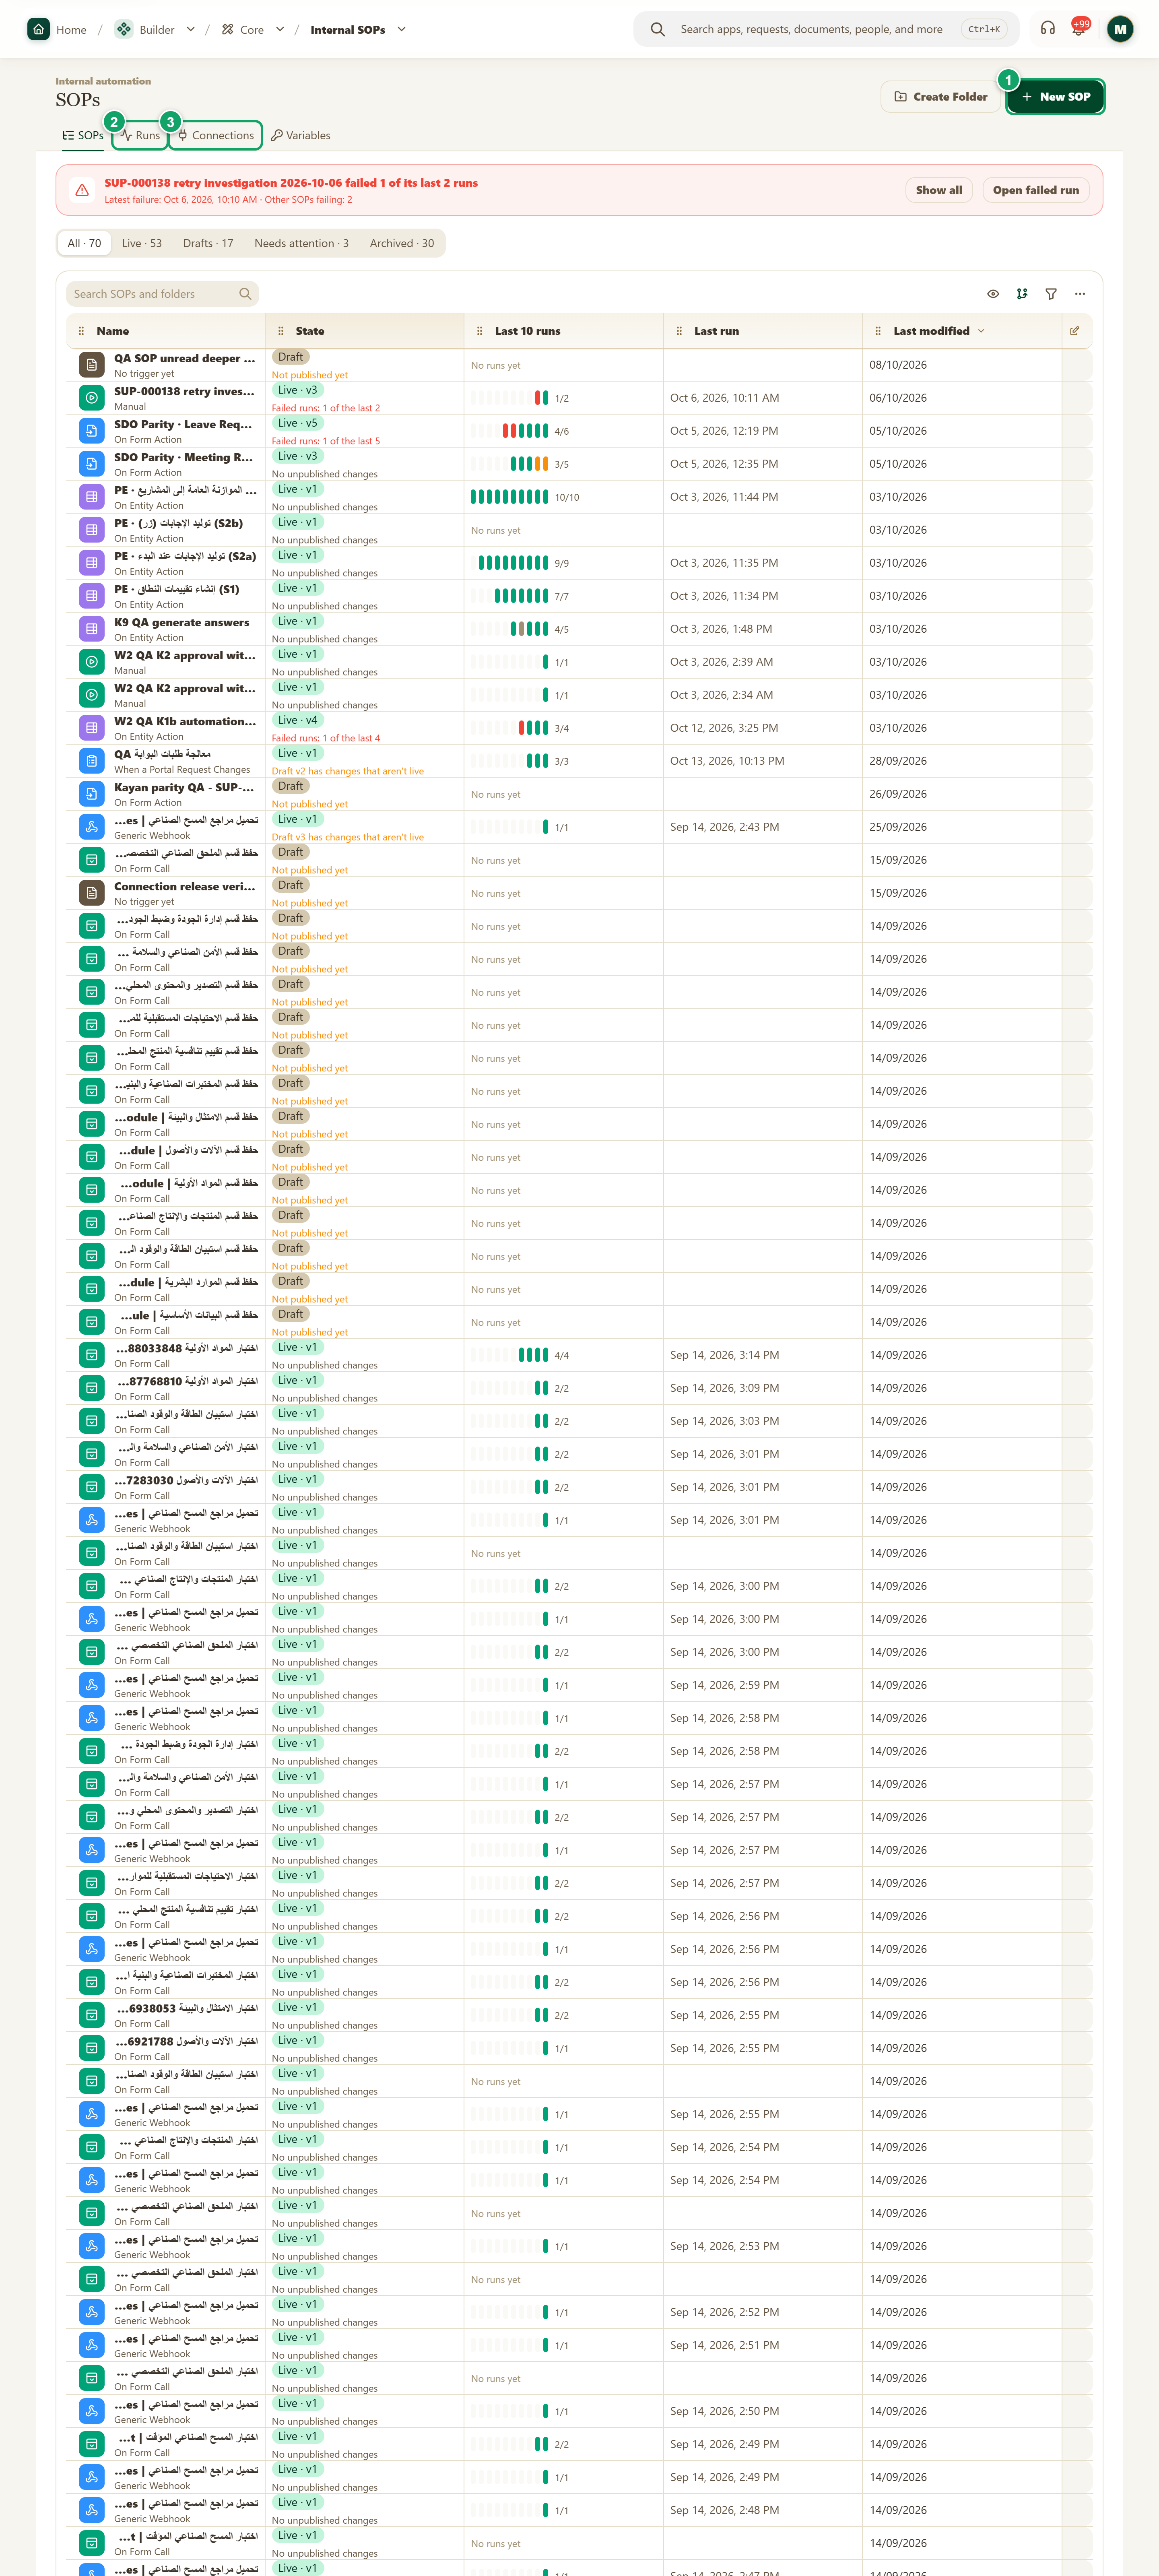
\includegraphics[width=0.95\linewidth,height=0.72\textheight,keepaspectratio]{figures/screens/ch06-internal-sops-en.png}
\caption{The “Internal SOPs” page}
\label{fig:builder-internal-sops-screen}
\shotnote{The page lists SOPs, their states and follow-up tabs. The list is empty in the test organization. ① “New SOP”: starts an SOP and asks what starts it. ② “Runs”: every time an SOP ran and its result. ③ “Connections”: external service accounts the steps use.}
\end{figure}


\begin{table}[H]
\centering
\caption{What do you find here?}
\label{tab:builder-internal-sops-data}
\begin{tabularx}{\linewidth}{R{3.6cm} Y}
\rcHeaderRow
\thh{Tab or tool} & \thh{Content and action}\\
SOPs & The list of SOPs with their state and recent run results, filtered by “Live”, “Drafts”, “Needs attention”, “Paused” and “Archived”.\\
Runs & Every time an SOP started, with its status: queued, running, waiting, completed or failed.\\
Connections and Variables & External service accounts the steps use, and encrypted values SOPs can use.\\
New SOP & Write the name and choose “What starts it?”, such as “On Form Submitted”, “New Record Created”, “Schedule” or “Manual”, then “Create and open”.\\
Editor & The step canvas with “Build”, “Test” and “Runs” modes. Steps include approval, form and signature requests, task creation, decisions, waits, and creating or updating records.\\
Review \& publish & Shows what to fix and the changes since the live version, then publishes a new version. Runs in progress finish on their old version.\\
\end{tabularx}
\end{table}

\begin{figure}[H]
\centering
\begin{tikzpicture}[node distance=0.5cm]
\node[stepBox] (a) {Trigger: what starts it?};
\node[stepBox,below=of a] (b) {Human and automatic steps};
\node[stepBox,below=of b] (c) {Test: safe simulation};
\node[stepBox,below=of c] (d) {Review and publish};
\node[stepBox,below=of d] (e) {Follow the runs};
\draw[flowsTo] (a) -- (b);
\draw[flowsTo] (b) -- (c);
\draw[flowsTo] (c) -- (d);
\draw[flowsTo] (d) -- (e);
\end{tikzpicture}
\rclegend
\caption{The life of an internal SOP}
\label{fig:builder-internal-sops-flow}
\shotnote{The diagram shows that an SOP runs only after it is published, and that testing comes before publishing. “Simulate (safe)” creates nothing real and makes external steps return example data, so you test the path without disturbing anyone. After publishing, follow the runs to see where the SOP succeeded and where it stopped.}
\end{figure}

\subsection{Steps and check}
\begin{enumerate}
\item Open “Internal SOPs”, press “New SOP”, name it, choose what starts it and press “Create and open”.
\item Add the steps on the canvas and finish setting up each one until “All steps ready” appears.
\item Switch to “Test” mode, choose “Simulate (safe)”, then press “Run simulation”.
\item Press “Review \& publish”, review the changes, then publish the version.
\end{enumerate}

\textbf{Check and recovery:} the SOP's state should be “Live”, and runs should appear after the event happens. If a run fails, open it from “Runs” to see the failed step, fix it and publish again. To stop the SOP for a while, pause it instead of deleting it; no new runs start until you resume it.
